\documentclass[a4paper,11pt,twoside]{scrreprt}

\usepackage[utf8]{inputenc}
\usepackage[T1]{fontenc}   
\usepackage{graphicx}       
\usepackage[german]{babel}
\usepackage{csquotes}     
\usepackage{acronym}
\usepackage{eurosym}
\usepackage[linktocpage=true]{hyperref}
\usepackage[bindingoffset=8mm]{geometry}
\usepackage{caption}
\captionsetup{format=hang, justification=raggedright}
\usepackage[style=authoryear, backend=biber]{biblatex}
\usepackage{float}
\usepackage{rotating}
\usepackage{blkarray}
\usepackage{amsmath}
\usepackage{amssymb}
\usepackage{gensymb}
\usepackage{amsthm}
\newtheorem{theorem}{Theorem}[section]
\newtheorem{lemma}[theorem]{Lemma}
\usepackage{listings}
\addbibresource{references.bib} 
\usepackage{caption}
\usepackage{subcaption}
\usepackage{interval}


\newcommand{\argmin}[1]{\underset{#1}{\operatorname{arg}\,\operatorname{min}}\;}
\newcommand{\norm}[1]{\lVert#1\rVert}
\newcommand{\Lagr}{\mathcal{L}}

\begin{document}

% Titelblatt:
% \newpage\mbox{}\newpage
\cleardoublepage   % force output to a right page
\thispagestyle{empty}
\begin{titlepage}
  \begin{flushright}
  
\includegraphics[width=0.4\linewidth]{assets/Logo-A3.jpg}
  \end{flushright}
  \begin{center}
  \section*{Support Vector Machines (SVM)}
  \vspace{2cm}

\textbf{Computational Intelligence II}    
\vspace{0.5cm}

  Informatik - Software and Information Engineering\\
  Fachhochschule Vorarlberg\\

  \vspace{1cm}
  
    Erstellt von\\
  André Hopfgartner \& Matthias Rupp\\
  
 
  \vspace{1cm}
  

  
  Dornbirn, am \today
  
  
  \end{center}
\end{titlepage}


% Inhaltsverzeichnis:
\clearpage   % force output to a right page
\setcounter{tocdepth}{2}
\setcounter{secnumdepth}{4}
\tableofcontents

% evtl. Abkürzungsverzeichnis:
\clearpage
\phantomsection
\addcontentsline{toc}{chapter}{Abkürzungsverzeichnis}
\chapter*{Abkürzungsverzeichnis}
\begin{acronym}
 \acro{SVM}{Support Vector Machine}
 \acro{QP}{Quadratic Programming}
\end{acronym}



\chapter{Einführung}

\section{Intuition}
Ziel: Ebene so wählen dass möglichst breites Band zwischen den 2 verschiedenen Klassen entsteht. \\

Hard Margin SVM: Trennebene trennt Daten, alle Eingabevektoren werden richtig klassifziert
Soft Margin SVM: Trennebene trennt Daten, Eingabevektoren können falsch klassifiziert werden, Fehlklassifikationen werden minimiert

\begin{figure}[H]
	\centering
	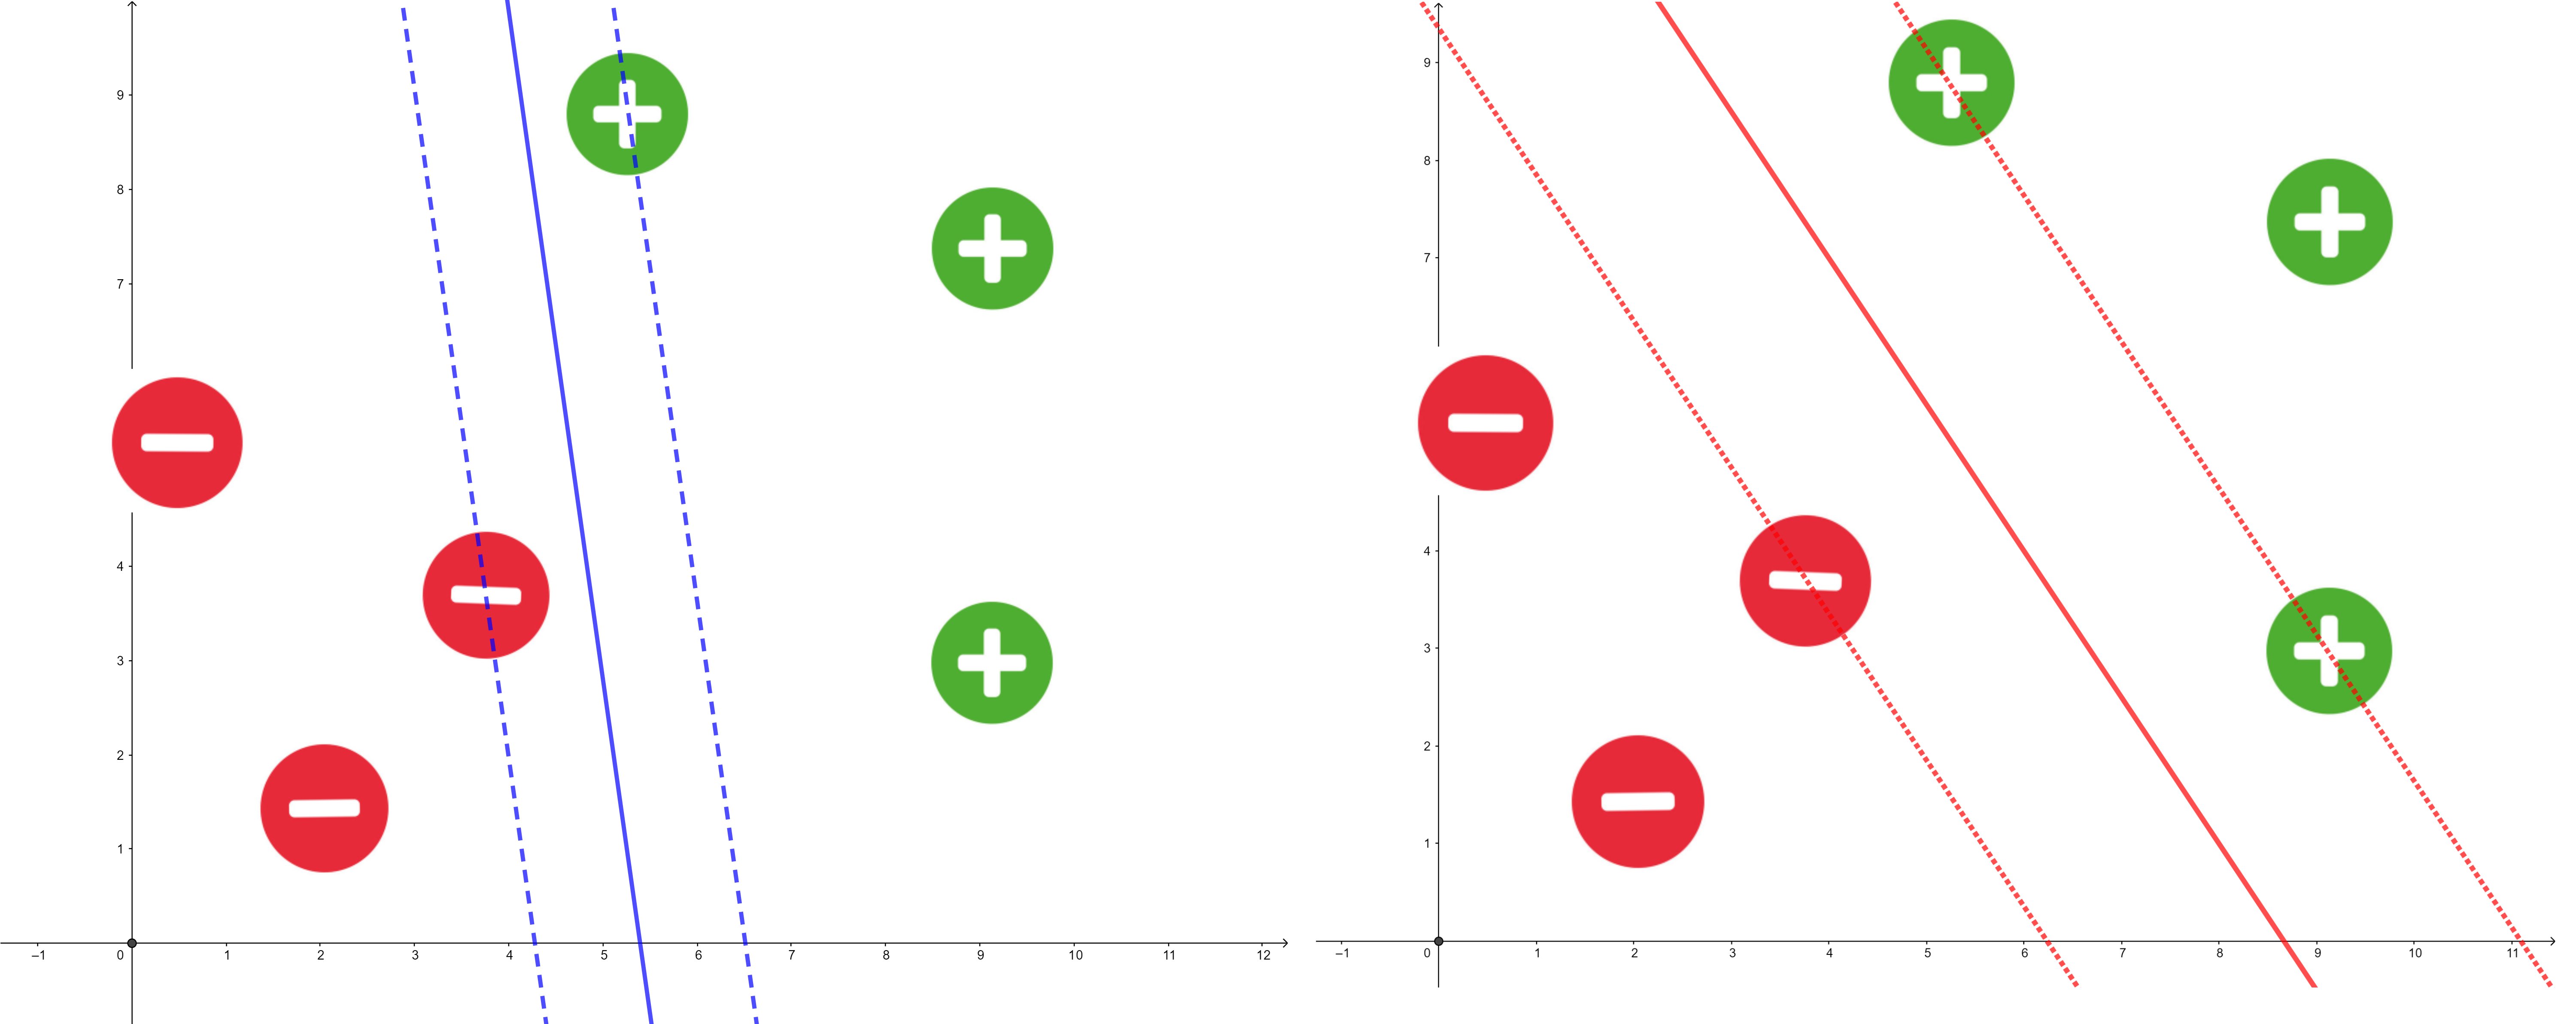
\includegraphics[width = 16cm]{assets/small_vs_big_margin.png}
	\caption{Abhängig von der Lage der Trennebene entstehen schmale (blau) oder breite (rot) Trennbänder. Das Ziel der \ac{SVM} ist die Maximierung der Breite des Trennbands durch die Ermittlung der optimalen Lage der Trennebene.}
	\label{fig:intuition_margin}
\end{figure}


\section{Hard-Margin Support Vector Machine} \label{sec:hard_margin}

TODO ZUSAMMENFASSUNG HERE

\subsection{Problemdefinition}
Gegeben sei ein Gewichtsvektor $w \in \mathbb{R}^{K}$, ein Bias $b \in \mathbb{R}$, ein beliebiger Punkt $x_{n} \in \mathbb{R}^{K}$ und ein zugehöriges Label $y_{n} \in \{\-1, +1\}$. Eine Ebene im Raum kann allgemein definiert werden durch:

\begin{equation} \label{plane_eq}
    \begin{aligned}
    w^{T} x_{n} + b &= 0 \\
    \end{aligned}
\end{equation}

Mit einer bereits trainierten \ac{SVM} können neue, noch unklassifizierte Eingabevektoren $x$ wie folgt klassifiziert werden:

\begin{subequations} \label{svm_classify1}
	\begin{alignat}{2}
		y = sign(w^{T} x + b)  & \qquad & \text{ gleichbedeutend mit} \\
		w^{T} x + b > 0 & & \text{ für } y = +1\\
		w^{T} x + b < 0 & & \text{ für } y = -1
	\end{alignat}
\end{subequations}


Für die Herleitung führen wir eine noch striktere Regel ein. So soll für eine richtige Klassifikation eines gegebenen Eingabevektors $x_{n}$ mit dem Label $y_{n}$ gelten:
\begin{subequations} \label{decision_rules}
	\begin{alignat}{2}
		w^{T} x_{n} + b \geq +1 & \qquad & \text{ für } y_{n} = +1\\
		w^{T} x_{n} + b \leq -1 & & \text{ für } y_{n} = -1
	\end{alignat}
\end{subequations}


Durch \autoref{decision_rules} wird sichergestellt, dass Werte aus dem Intervall $\interval[open]{-1}{+1}$ als Ergebnis nicht vorkommen können. Wie in \autoref{fig:trennband} dargestellt entsteht dadurch ein symmetrisches Trennband um die Trennebene in dem keine Punkte liegen. Ziel der \ac{SVM} ist die Maximierung der Breite dieses Bandes.\\

\begin{figure}[H]
	\centering
	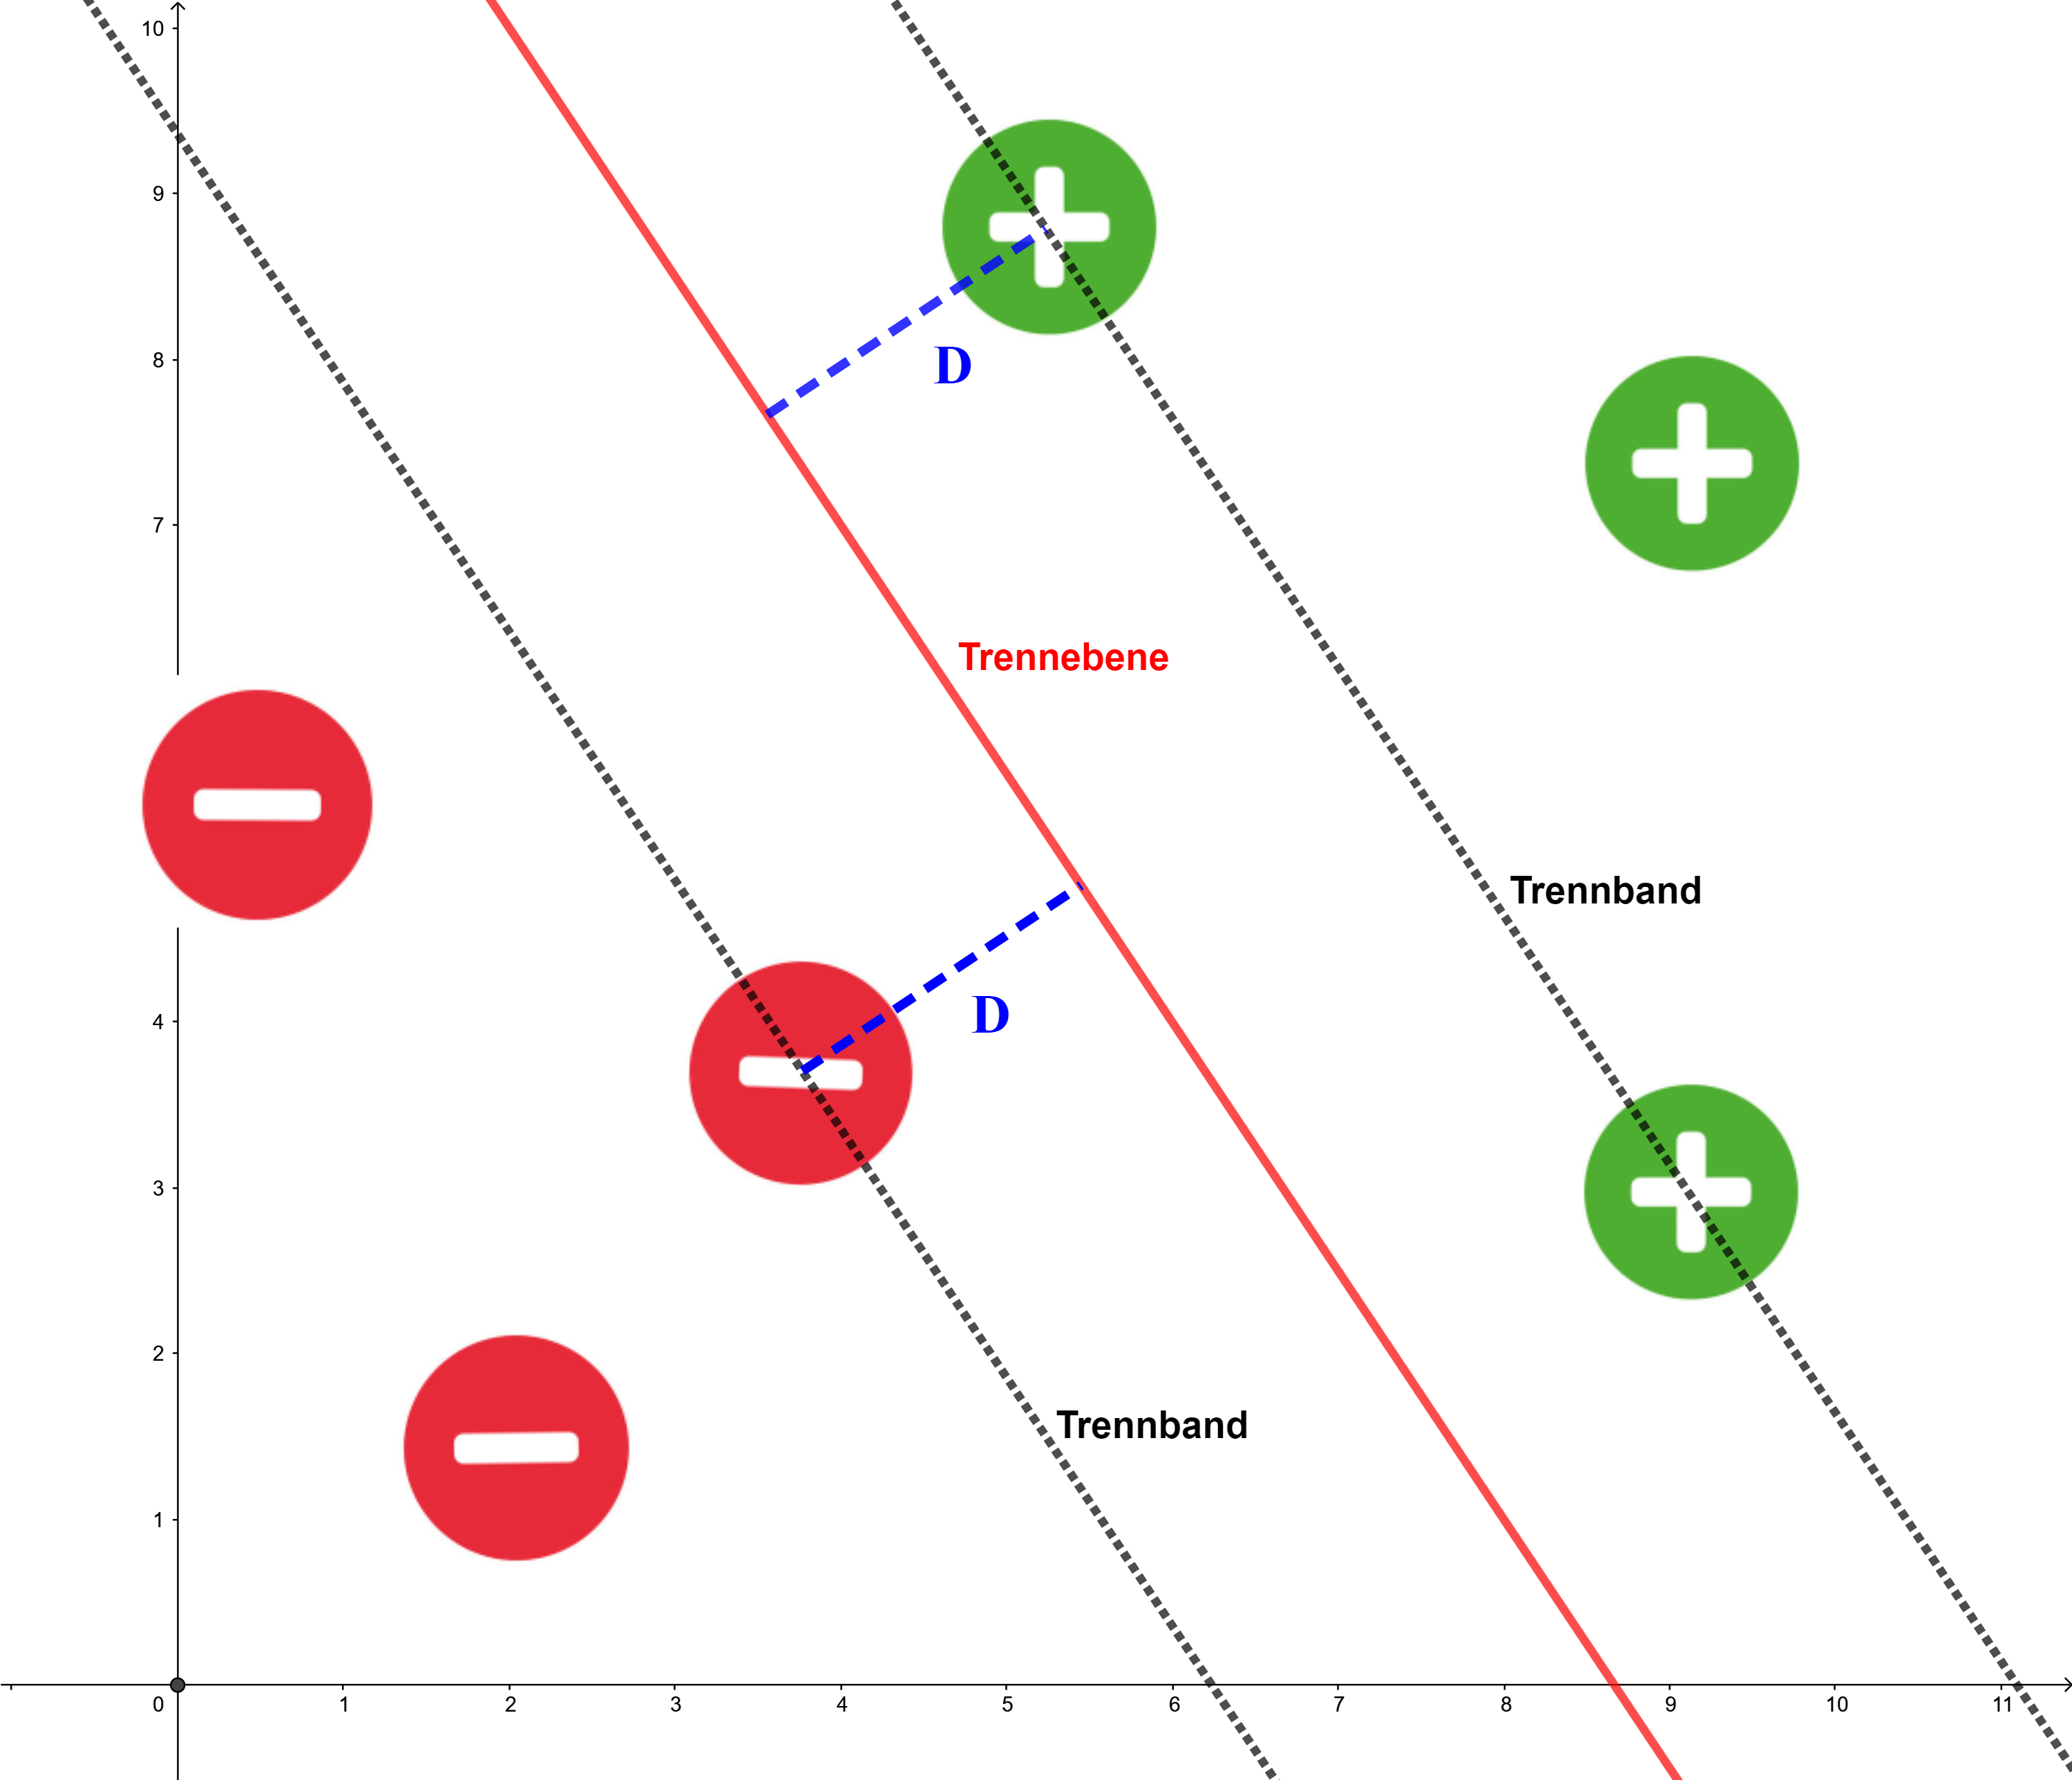
\includegraphics[width = 12cm]{assets/trennband.png}
	\caption{Um die Trennebene entsteht ein Trennband. Die am nächsten zu der Ebene liegenden Eingabevektoren liegen genau auf den Grenzen des Trennbands.}
	\label{fig:trennband}
\end{figure}



 \autoref{decision_rules} kann weiter verallgemeinert werden durch beidseitige Multiplikation mit $y_{k}$:

\begin{subequations} \label{decision_rules2}
	\begin{alignat}{2}
		y_{k} (w^{T} x_{n} + b) \geq 1 & \qquad & \text{ für } y_{k} = +1\\
		y_{k} (w^{T} x_{n} + b) \geq 1 & & \text{ für } y_{k} = -1
	\end{alignat}
\end{subequations}



Für den Fall, dass $x_{n} = \hat{x}$ genau an der Grenze des Trennbands liegt, gilt somit:
\begin{equation} \label{dec_rule}
	\begin{aligned}
		y_{k} (w^{T} \hat{x} + b) &= 1
	\end{aligned}
\end{equation}


Als nächsten Schritt bestimmen wir den euklidischen Normalabstand $D$ eines beliebigen Punkts $x_{n} \in \mathbb{R}^{K}$ zu der Ebene. Hierfür ist zuerst zu bemerken, dass $w$ normal zur definierten Ebene steht.

\begin{lemma}
	Eine Ebene sei definiert durch $w^{T} x + b = 0$. Der Vektor $w$ steht normal zu der definierten Ebene.
\end{lemma}

\begin{proof}
	Man wähle zwei Punkte $x_{1}, x_{2} \in \mathbb{R}^{K}$ die auf der Ebene liegen. Somit muss gelten:
	\begin{equation}
		\begin{aligned}
			w^{T} x_{1} + b &= 0 \\
			w^{T} x_{2} + b &= 0 \\
			w^{T} (x_{1} - x_{2}) &= 0 \leftrightarrow \norm{w^{T}} \norm{x_{1} - x_{2}} \cos(\alpha) = 0 \leftrightarrow \alpha = 90^{\circ}
		\end{aligned}
	\end{equation}
\end{proof}

Um den Normalabstand $d$ eines beliebigen Punkts $x_{n}$ zu ermitteln wählt man einen Punkt $x$, der auf der Ebene liegt, und projiziert den Vektor $(x_{n} - x)$ auf den Einheitsvektor von $w$. Weil nur der tatsächliche Abstand zur Ebene relevant ist und nicht die Richtung nimmt man den Betrag.

\begin{equation} \label{distance_to_plane}
	\begin{aligned}
		d &= | \frac{w^{T}}{\lVert w \rVert} (x_{n} - x) | = \\
		&= \frac{1}{\norm{w}} | (w^{T} x_{n} - w^{T} x) | =\\
		&= \frac{1}{\norm{w}} | (w^{T} x_{n} + b - (w^{T} x + b)) |
	\end{aligned}
\end{equation}

\begin{figure}[H]
	\centering
	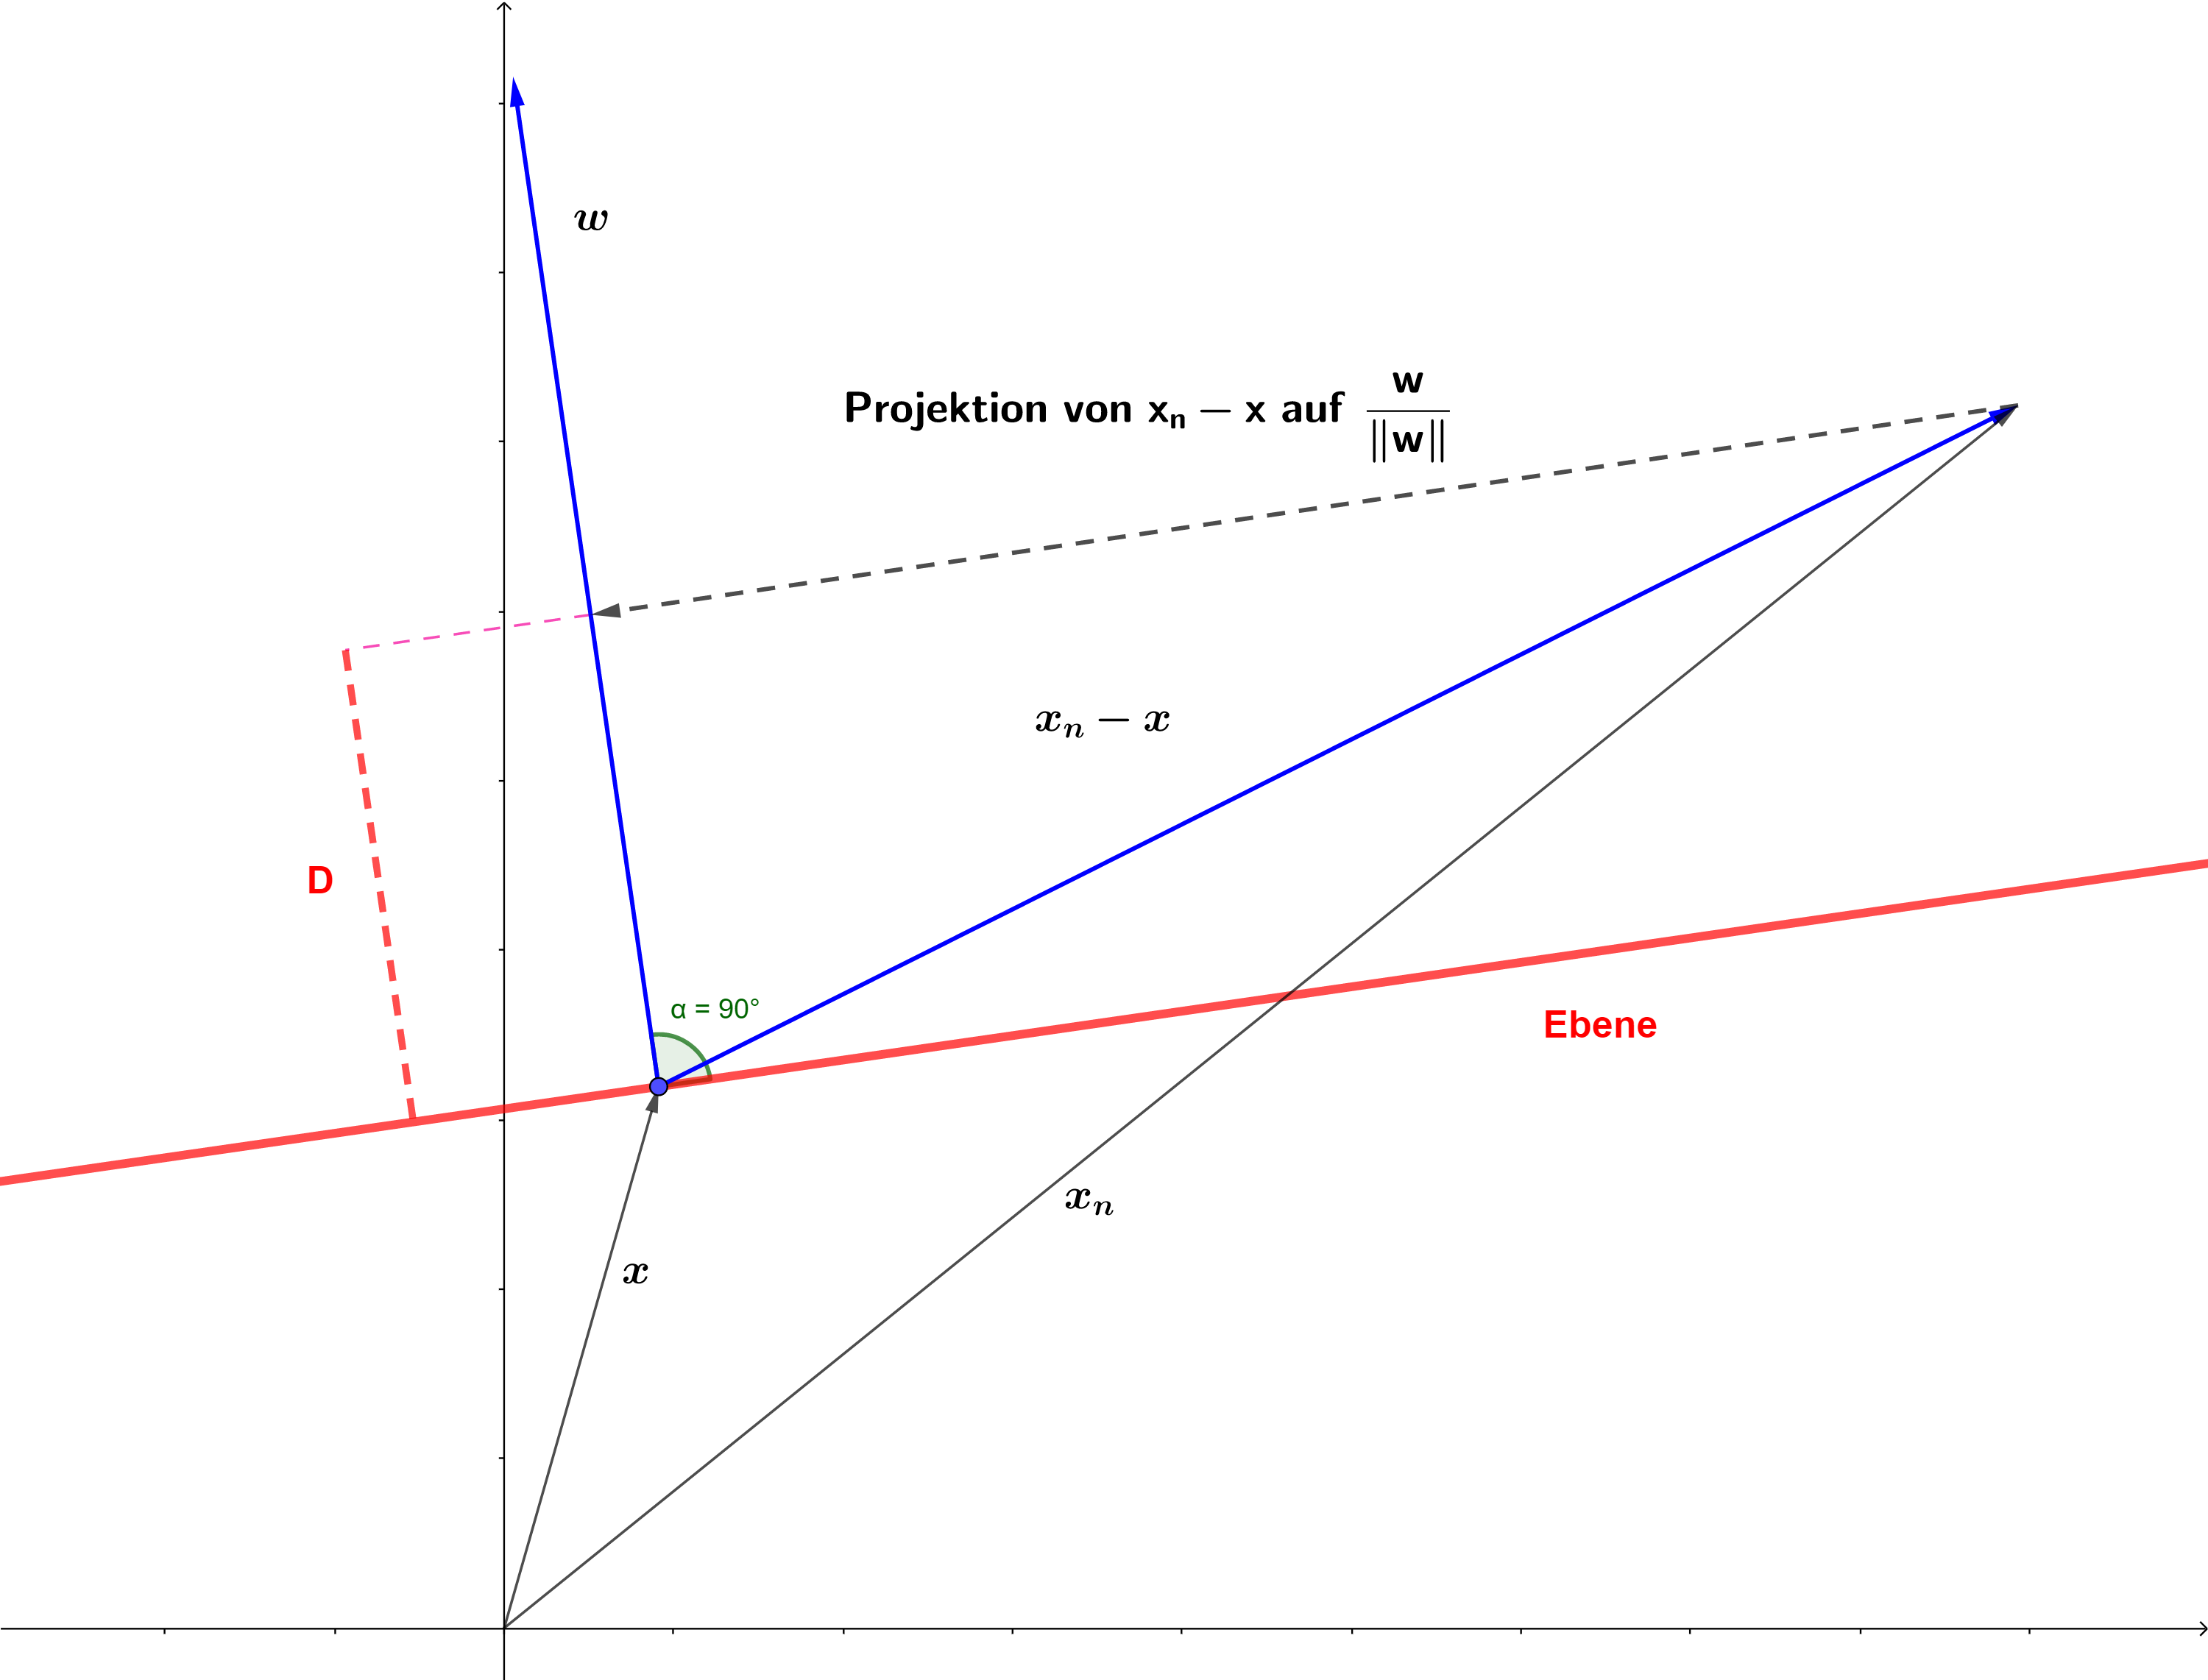
\includegraphics[width = 13cm]{assets/projection.png}
	\caption{Durch die Projektion von $(x_{n} - x)$ auf den Einheitsvektor von $w$ kann der Normalabstand $d$ von $x_{n}$ zu der Ebene bestimmt werden.}
	\label{fig:projection}
\end{figure}

Weil der Punkt $x$ auf der Ebene liegt gilt $w^{T} x + b = 0$ (\autoref{plane_eq}):
\begin{equation} \label{distance_to_plane_simplified1}
	\begin{aligned}
		d &= \frac{1}{\norm{w}} | (w^{T} x_{n} + b) |
	\end{aligned}
\end{equation}

Trifft man nun die Annahme, dass $x_{n} = \hat{x}$ der am nächsten zu der Trenngrenze liegende Punkt ist, so gilt aus \autoref{dec_rule} gilt $y_{k} (w^{T} \hat{x} + b) = 1 = |w^{T} \hat{x} + b|$ unter der Annahme, dass der Punkt richtig klassifiziert wurde. Somit ergibt sich der kleinste Abstand zur Trennebene $D = d(\hat{x})$, welcher zugleich der halben Breite des Trennbands entspricht, als:
\begin{equation} \label{distance_to_plane_simplified2}
	\begin{aligned}
		D &= \frac{1}{\norm{w}}
	\end{aligned}
\end{equation}

\begin{figure}[H]
	\centering
	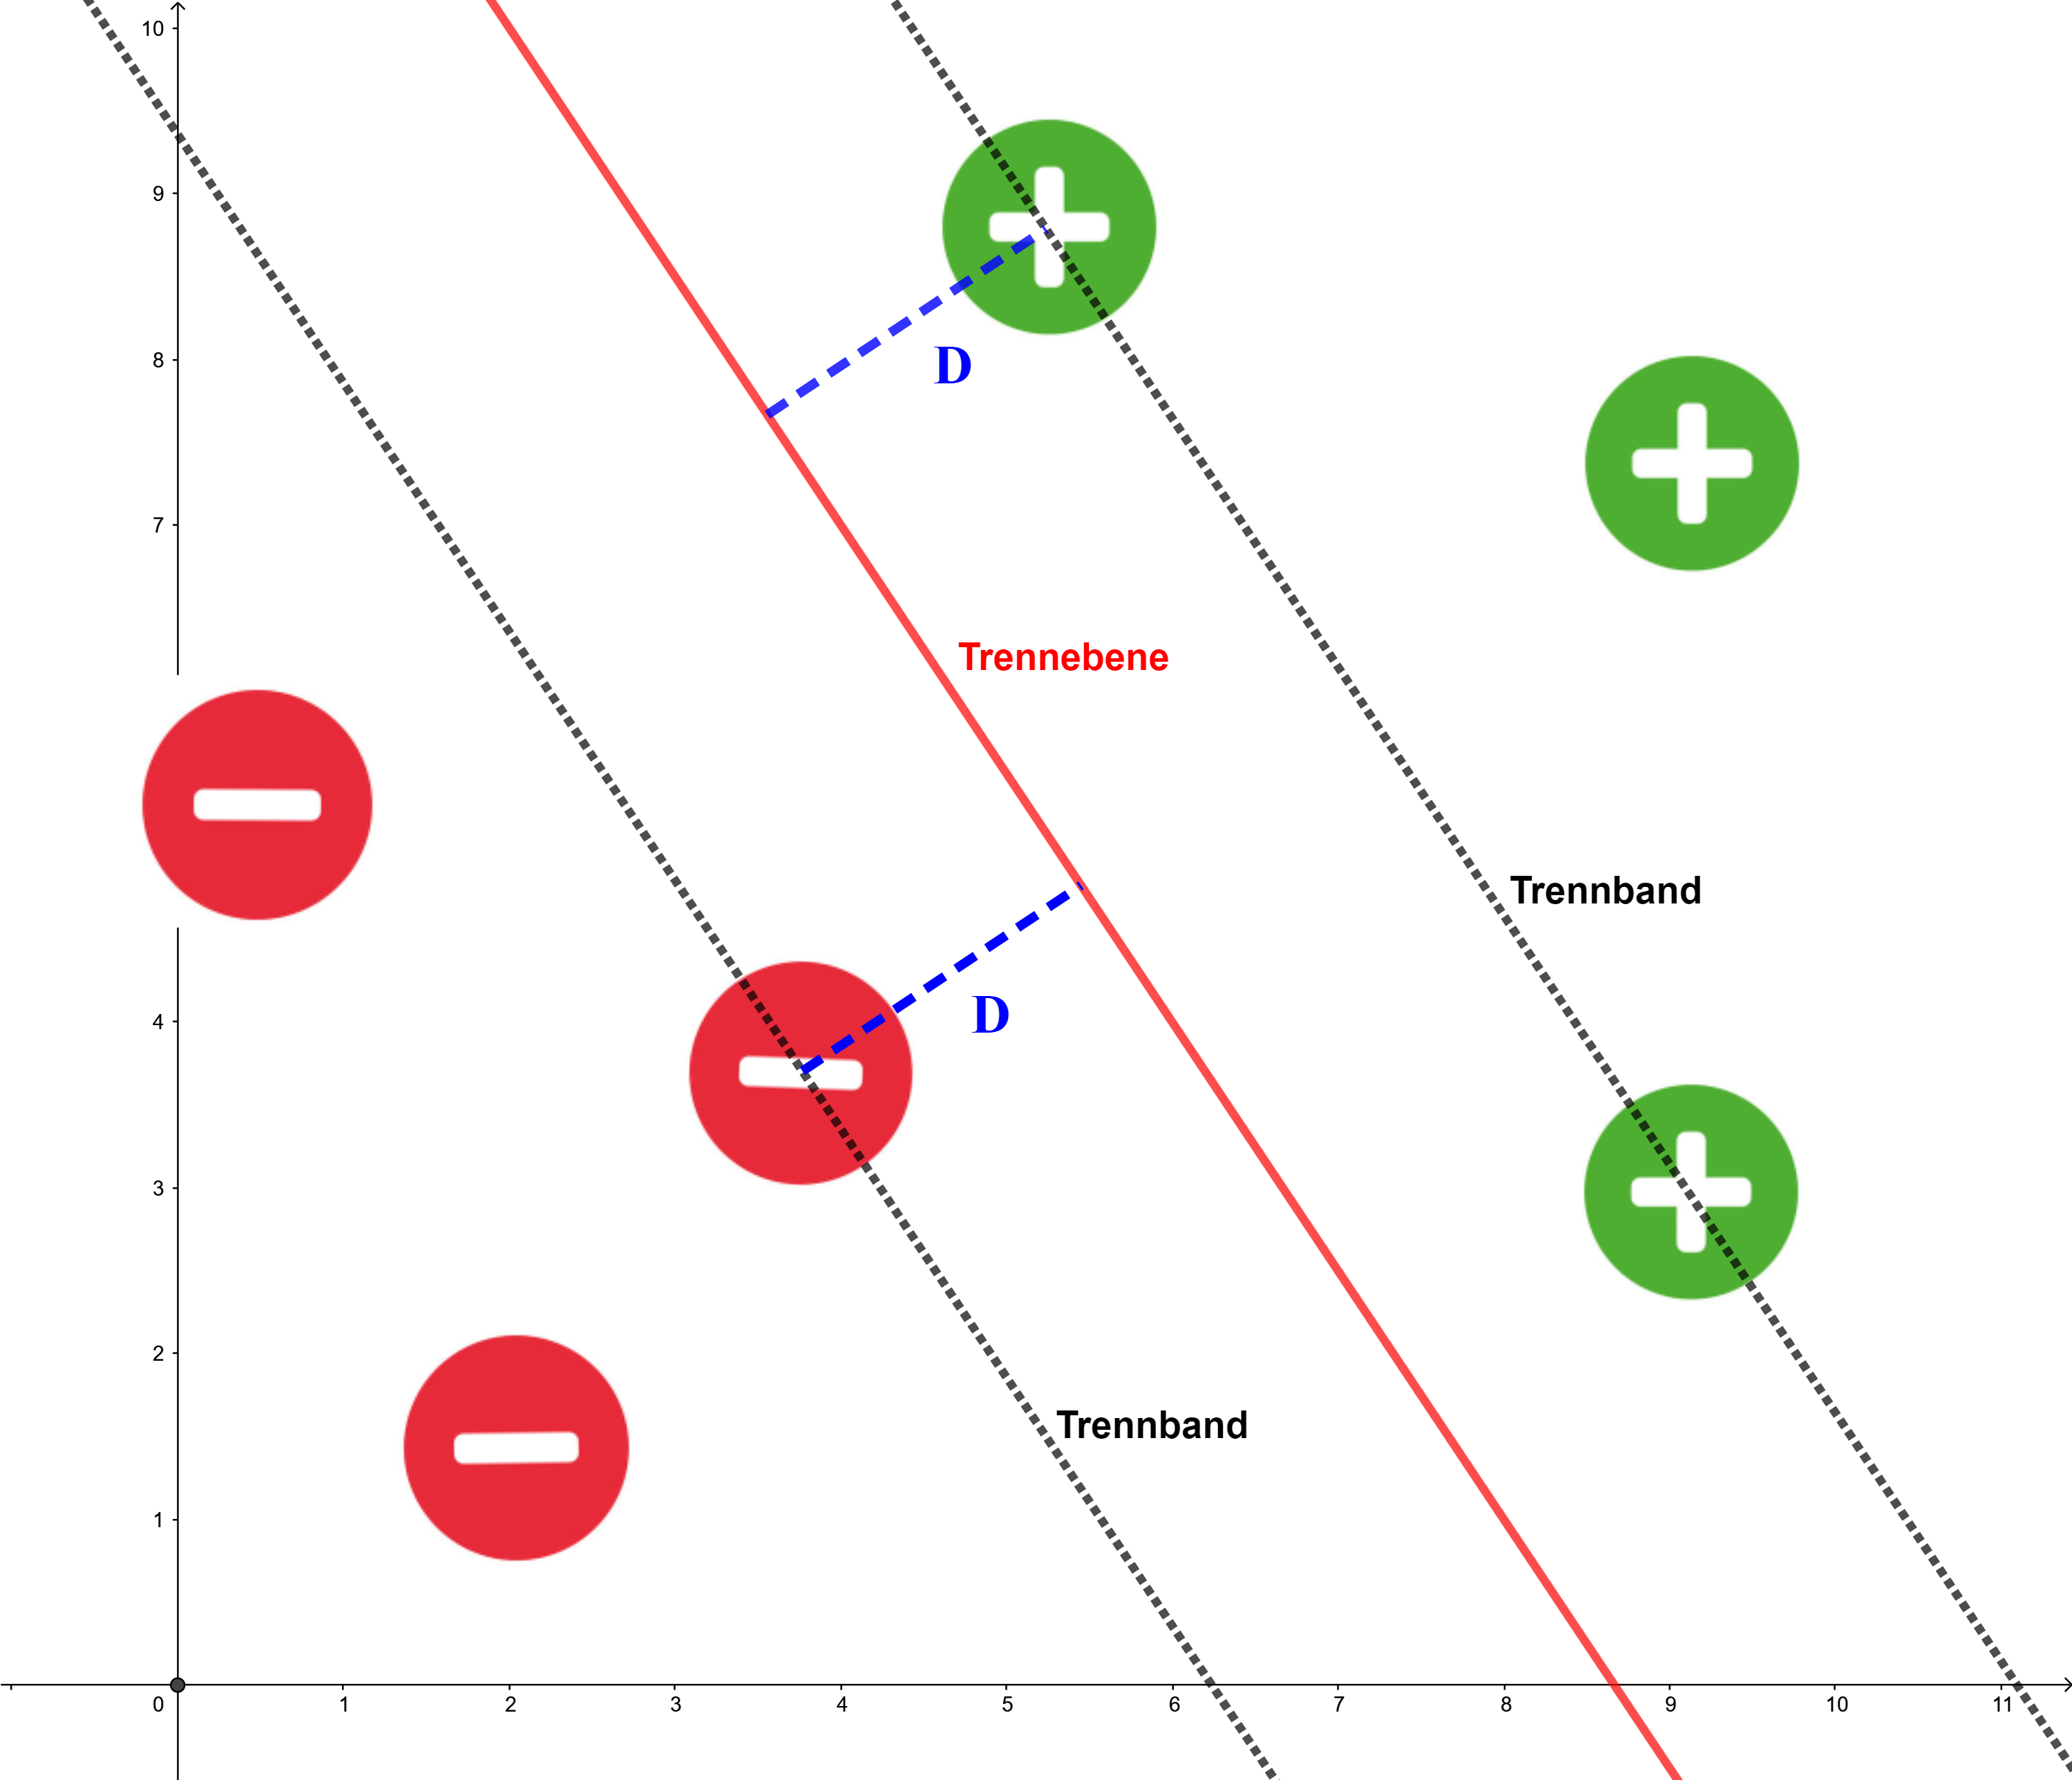
\includegraphics[width = 12cm]{assets/trennband_mit_D.png}
	\caption{Der Normalabstand $D$ von der Ebene zu den am nächsten liegenden Eingabevektoren entspricht genau der Hälfte der Breite des Trennbands.}
	\label{fig:trennband2}
\end{figure}


\subsection{Optimierungsproblem}

\autoref{distance_to_plane_simplified2} beschreibt den Normalabstand zu dem am nächsten an der Ebene liegenden Punkt $\hat{x}$. Der Normalabstand ist gleichbedeutend mit der Hälfte der Breite des Trennbands, wobei für die Optimierung der Faktor $2$ keine Rolle spielt und vernachlässigt werden kann. \\
Das Ziel einer \ac{SVM} ist die Maximierung der Breite des Trennbands für $N$ Eingabevektoren $\{x_{1}..x_{N}\}, x_{n} \in \mathbb{R}^{K}$. Bei der in diesem Kapitel hergeleiteten Version der \ac{SVM} müssen die Eingabevektoren linear separierbar sein. Diese Art der \ac{SVM} wird auch Hard-Margin SVM genannt. Die zweite Version, bei der nicht alle Eingabevektoren linear trennbar sind, heißt Soft-Margin SVM und wird in \autoref{sec:soft_margin} beschrieben. \\

Bei dem beschriebenen Problem handelt es sich um ein Optimierungsproblem mit Nebenbedingungen:

\begin{subequations}
	\begin{alignat}{2}
		&\!\max_{w}        &\qquad&  \frac{1}{\norm{w}} \label{eq:optProb}\\
		&\text{mit } &      & \min_{n=1..N} |w^{T} x_{n} + b| = 1 \label{eq:constraint1}
	\end{alignat}
\end{subequations}

\autoref{eq:constraint1} beschreibt hier den am nächsten zur Ebene gelegenen Punkt $\hat{x}$ aus der gebenenen Menge von Eingabevektoren in allgemeiner Form. Der Betrag lässt sich vermeiden durch die Anwendung von \autoref{decision_rules2}:

\begin{equation} \label{abs_value_trick}
	\begin{aligned}
		|w^{T} x_{n} + b| &= y_{n} (w^{T} x_{n} + b)
	\end{aligned}
\end{equation}


Durch Anwendung von \autoref{abs_value_trick} in \autoref{eq:constraint1}, Umformulierung der Maximierung in eine Minimierung und der Verallgemeinerung von $\hat{x}$ auf beliebige Punkte $x_{n}$ erhält man:
\begin{subequations}
	\begin{alignat}{2}
		&\!\min_{w}        &\qquad&  \frac{1}{2} w^{T} w \label{eq:optProb2}\\
		&\text{mit } &      & y_n (w^{T} x_{n} + b) \geq 1 \text{ für } n=1..N \label{eq:constraint12}
	\end{alignat}
\end{subequations}

Die Verallgemeinerung von \autoref{eq:constraint1} auf \autoref{eq:constraint12} auf beliebige Punkte ist so möglich, weil durch \autoref{dec_rule} sichergestellt ist, dass für beliebige Punkte $y_{n}(w^{T} x_{n} + b) \geq 1$ gilt.

\subsection{Lagrange Optimierung} \label{sec:lagrange}

Das beschriebene Optimierungsproblem beinhaltet eine Ungleichung in \autoref{eq:constraint12}. Um die Lagrangegleichung aufstellen zu können wird zuerst die Nebenbedingung umgeformt:
\begin{subequations} \label{min_problem}
	\begin{alignat}{2}
		&\!\min_{w}        &\qquad&  \frac{1}{2} w^{T} w \label{eq:optProb3}\\
		&\text{mit } &      & y_n (w^{T} x_{n} + b)-1 \geq 0 \text{ für } n=1..N \label{eq:constraint13}
	\end{alignat}
\end{subequations}

Das Problem kann nun als Lagrangegleichung dargestellt werden:
\begin{subequations}
	\begin{alignat}{2}
		&\!\min_{w, b}        &\qquad&  \Lagr (w, b, \alpha) = \frac{1}{2} w^{T} w - \sum_{n=1}^{N} \alpha_{n} (y_n (w^{T} x_{n} + b)-1) \label{eq:optProb4}\\
		&\max_{\alpha_{n}} &      & \alpha_{n} \geq 0 \text{ für } n=1..N \label{eq:constraint14}
	\end{alignat}
\end{subequations}
 Weil \autoref{eq:constraint13} eine Ungleichung der Form $\geq 0$ beinhaltet werden diese Terme von der zu maximierenden Funktion subtrahiert. Nun kann die uneingeschränkte Optimierung von \autoref{eq:optProb4} nach $w$ und $b$ durchgeführt werden indem die Ableitungen bestimmt und $0$ gesetzt werden:

\begin{equation} \label{gradient_lagrange_w}
	\begin{aligned}
		\nabla_{w} \Lagr &= w - \sum_{n=1}^{N} \alpha_{n} y_{n} x_{n} \overset{!}{=} \vec{0} \\
		w &= \sum_{n=1}^{N} \alpha_{n} y_{n} x_{n}
	\end{aligned}
\end{equation}

\begin{equation} \label{partial_lagrange_b}
	\begin{aligned}
		\frac{\partial}{\partial b} \Lagr &= - \sum_{n=1}^{N} \alpha_{n} y_{n} \overset{!}{=} 0 \\
		\sum_{n=1}^{N} \alpha_{n} y_{n} &= 0
	\end{aligned}
\end{equation}

Die Ergebnisse von \autoref{gradient_lagrange_w} und \autoref{partial_lagrange_b} können in \autoref{eq:optProb4} eingesetzt werden. Hierfür wird zuerst die Summe in \autoref{eq:optProb4} in Teilsummen aufgeteilt:

\begin{equation} \label{lagrange_substituted}
	\begin{aligned}
		\Lagr(w, b, \alpha) &= \frac{1}{2} w^{T} w - \sum_{n=1}^{N} \alpha_{n} (y_n (w^{T} x_{n} + b)-1) = \\
		&= \frac{1}{2} w^{T} w - [\sum_{n=1}^{N} \alpha_{n} y_{n} b - \sum_{n=1}^{N} \alpha_{n} + \sum_{n=1}^{N} \alpha_{n} y_{n} w^{T} x_{n}]
	\end{aligned}
\end{equation}

Weil $\sum_{n=1}^{N} \alpha_{n} y_{n} = 0$ (\autoref{partial_lagrange_b}) gilt fällt der Term $\sum_{n=1}^{N} \alpha_{n} y_{n} b$ weg:
\begin{equation} \label{lagrange_substituted2}
	\begin{aligned}
		\Lagr(w, b, \alpha) &= \frac{1}{2} w^{T} w - [-\sum_{n=1}^{N} \alpha_{n} + \sum_{n=1}^{N} \alpha_{n} y_{n} w^{T} x_{n}]
	\end{aligned}
\end{equation}

Vergleicht man den Term $\sum_{n=1}^{N} \alpha_{n} y_{n} w^{T} x_{n}$ mit dem Ergebnis von \autoref{gradient_lagrange_w} erkennt man, dass $\sum_{n=1}^{N} \alpha_{n} y_{n} w^{T} x_{n} = w^T w$ gilt. Dies kann ausgeschrieben werden als:
\begin{equation} \label{lagrange_substituted3}
	\begin{aligned}
		\Lagr(\alpha) &= \sum_{n=1}^{N }\alpha_{n} - \frac{1}{2} \sum_{n=1}^{N} \sum_{m=1}^{M} y_{n} y_{m} \alpha_{n} \alpha_{m} x_{n}^{T} x_{m}
	\end{aligned}
\end{equation}

\autoref{lagrange_substituted3} beschreibt das Optimierungsproblem ohne Abhängigkeit von $w$ und $b$, wir haben jetzt also eine Maximierung für $\alpha$ mit Nebenbedingungen:
\begin{subequations} \label{final_lagrange}
	\begin{alignat}{2}
		&\!\max_{\alpha}        &\qquad&  	\Lagr(\alpha) = \sum_{n=1}^{N} \alpha_{n} - \frac{1}{2} \sum_{n=1}^{N} \sum_{m=1}^{M} y_{n} y_{m} \alpha_{n} \alpha_{m} x_{n}^{T} x_{m} \label{eq:optProb5}\\
		&\text{mit } &      & \alpha_{n} \geq 0 \text{ für } n=1..N \label{eq:constraint16}\\
		&       & & \sum_{n=1}^{N} \alpha_{n} y_{n} = 0\text{ für } n=1..N \label{eq:constraint17}
	\end{alignat}
\end{subequations}

Bei dem in \autoref{final_lagrange} beschriebene Problem handelt es sich um ein Quadratic Programming Problem, ersichtlich an dem Term $x_{n}^{T} x_{m}$, welches beispielsweise mittels eines Quadratic Programming Solvers gelöst werden kann. Als Ergebnis erhält man einen Vektor $\alpha$ mit allen $\alpha_{n}$. Durch Einsetzen in $w = \sum_{n=1}^{N} \alpha_{n} y_{n} x_{n}$ kann $w$ bestimmt werden. \\

Betrachtet man den Ergebnisvektor $\alpha$ so wird man feststellen, dass sehr viele Werte $0$ ergeben. In \autoref{eq:optProb4} befindet sich der Term $\alpha_{n} (y_n (w^{T} x_{n} + b)-1)$. Der Term $(y_n (w^{T} x_{n} + b)-1)$ kann als Schlupf bezeichnet werden. Das Produkt von Schlupf und $\alpha_{n}$ kann nur $0$ werden wenn entweder der Schlupf $0$ ist oder $\alpha_{n}$. Umgekehrt bedeutet dies, dass alle Vektoren, die einen minimalen Abstand zu der Trennebene haben, ein $\alpha_{n} \neq 0$ aufweisen. Vektoren, die diese Bedingung erfüllen, werden Stützvektoren genannt. \\


Mit dieser Erkenntnis kann \autoref{gradient_lagrange_w} erneut analysiert werden:

\begin{equation} \label{weights_calc}
	\begin{aligned}
		w &= \sum_{n=1}^{N} \alpha_{n} y_{n} x_{n}
	\end{aligned}
\end{equation}

Weil nur Stützvektoren ein $\alpha_{n} \neq 0$ aufweisen und somit auch nur Stützvektoren einen Beitrag zu $w$ leisten, kann \autoref{weights_calc} stark vereinfacht werden:

\begin{equation} \label{weights_calc2}
	\begin{aligned}
		w &= \sum_{n \text{ ist Stützvektor}} \alpha_{n} y_{n} x_{n}
	\end{aligned}
\end{equation}

Der Gewichtsvektor $w$ hängt also lediglich von den Stützvektoren ab, deren Anzahl in der Regel gering ist.\\


Noch offen ist die Bestimmung des Bias $b$. Weil für Stützvektoren $y_n (w^{T} x_{n} + b) = 1$ gilt (\autoref{dec_rule}) kann der Bias $b$ aus jedem beliebigen Stützvektor bestimmt werden:

\begin{equation} \label{bias_calc}
	\begin{aligned}
		b &= \frac{1}{y_{n}} - w^{T} x_{n}
	\end{aligned}
\end{equation}

\subsection{Lösung mittels Quadratic Programming Solver}

Weil es sich bei dem in \autoref{final_lagrange} beschriebene Optimierungsproblem um ein Quadratic Programming Problem handelt kann dieses auch mittels eines Quadratic Programming Solvers gelöst werden. Die Implementationsdetails für diese Lösungsverfahren werden an dieser Stelle nicht weiter ausgeführt. Für die Anwendung eines Quadratic Programming Solvers muss das Problem in die Standardform von \ac{QP} Problemen umformuliert werden.

\begin{equation} \label{std_QP_problem}
	\begin{aligned}
		\min_{x} &= \frac{1}{2} x^{T} Q x + c x + d 
	\end{aligned}
\end{equation}

$Q \in \mathbb{R}^{n \times n}$ ist eine symmetrische reelle Matrix mit Koeffizienten, die einen quadratischen Beitrag leisten. $c \in \mathbb{R}$ ist ein Faktor für den linearen Beitrag und $d \in \mathbb{R}$ ist ein fixer Anteil. \\

Unter der Voraussetzung, dass $\max_{x} f(x) = \min_{x} (-f(x))$ gilt können wir unser Maximierungsproblem aus \autoref{final_lagrange} in ein Minimierungsproblem umformen:
\begin{equation} \label{qp_adapt1}
	\begin{aligned}
		\min_{\alpha} \Lagr(\alpha) &= \frac{1}{2} \sum_{n=1}^{N} \sum_{m=1}^{M} y_{n} y_{m} \alpha_{n} \alpha_{m} x_{n}^{T} x_{m} - \sum_{n=1}^{N} \alpha_{n}
	\end{aligned}
\end{equation}

Als nächsten Schritt müssen wir die Koeffizienten aus den Summen extrahieren, $\alpha$ und $y$ als Vektor darstellen, das Problem in die Standard-QP-Form bringen und die Nebenbedingungen als Matrizenmultiplikation darstellen:


\begin{subequations} \label{qp1}
	\begin{alignat}{2}
		&\!\min_{\alpha}        &\qquad& \Lagr(\alpha) = \frac{1}{2} \alpha^{T} Q \alpha + (-1^T) \alpha \label{eq:qp1}\\
		&\text{mit} &      & Q = \begin{bmatrix} 
			y_{1}y_{1}x_{1}^{T}x_{1} & y_{1}y_{2}x_{1}^{T}x_{2} & \dots & y_{1}y_{N}x_{1}^{T}x_{N}\\
			y_{2}y_{1}x_{2}^{T}x_{1} & y_{2}y_{2}x_{2}^{T}x_{2} & \dots & y_{2}y_{N}x_{2}^{T}x_{N}\\
			\vdots & \vdots & \vdots & \vdots\\
			y_{N}y_{1}x_{N}^{T}x_{1} & y_{N}y_{2}x_{N}^{T}x_{2} & \dots & y_{N}y_{N}x_{N}^{T}x_{N}\\ 
	\end{bmatrix}\\
&\text{für} & & y^{T} \alpha = 0\\
& & & 0 \leq \alpha \leq \infty
	\end{alignat}
\end{subequations}

An dieser Stelle ist zu bemerken dass es sich bei der Matrix $Q$ um eine $N \times N$ Matrix handelt. Für eine große Anzahl an Trainingsdaten ist dies sehr problematisch beziehungsweise nicht mehr lösbar. Hier können andere Optimierungsverfahren wie beispielsweise in \textcite{platt_sequential_1998} beschrieben verwendet werden. \\


Das Problem in dieser Darstellung können wir direkt an ein Quadratic-Programming Solver Framework übergeben und erhalten einen Vektor $\alpha = (\alpha_{1}, \alpha_{2}, ..., \alpha_{n})$ als Ergebnis. \\

Daraus können wir, wie bereits zuvor erwähnt, $w$ und $b$ bestimmen:

\begin{equation} \label{weights_calc_qp}
	\begin{aligned}
		w &= \sum_{n=1}^{N} \alpha_{n} y_{n} x_{n}
	\end{aligned}
\end{equation}

Für die Biasberechnung benötigen wir einen beliebigen Stützvektor $x_{k}$. Wir finden einen Stützvektor, indem wir den Ergebnisvektor $\alpha$ betrachten. Ein Stützvektor $x_{k}$ muss $\alpha_{k} \neq 0$ aufweisen.
\begin{equation} \label{bias_calc_qp}
	\begin{aligned}
		b &= \frac{1}{y_{k}} - w^{T} x_{k}
	\end{aligned}
\end{equation}

Die \ac{SVM} ist nun vollständig definiert, neue Eingabevektoren $x$ können wie folgt klassifiziert werden:
\begin{equation} \label{svm_classify}
	\begin{aligned}
		y &= sign(w^{T} x + b)
	\end{aligned}
\end{equation}

\section{Soft-Margin Support Vector Machine} \label{sec:soft_margin}
\begin{figure}[H]
	\centering
	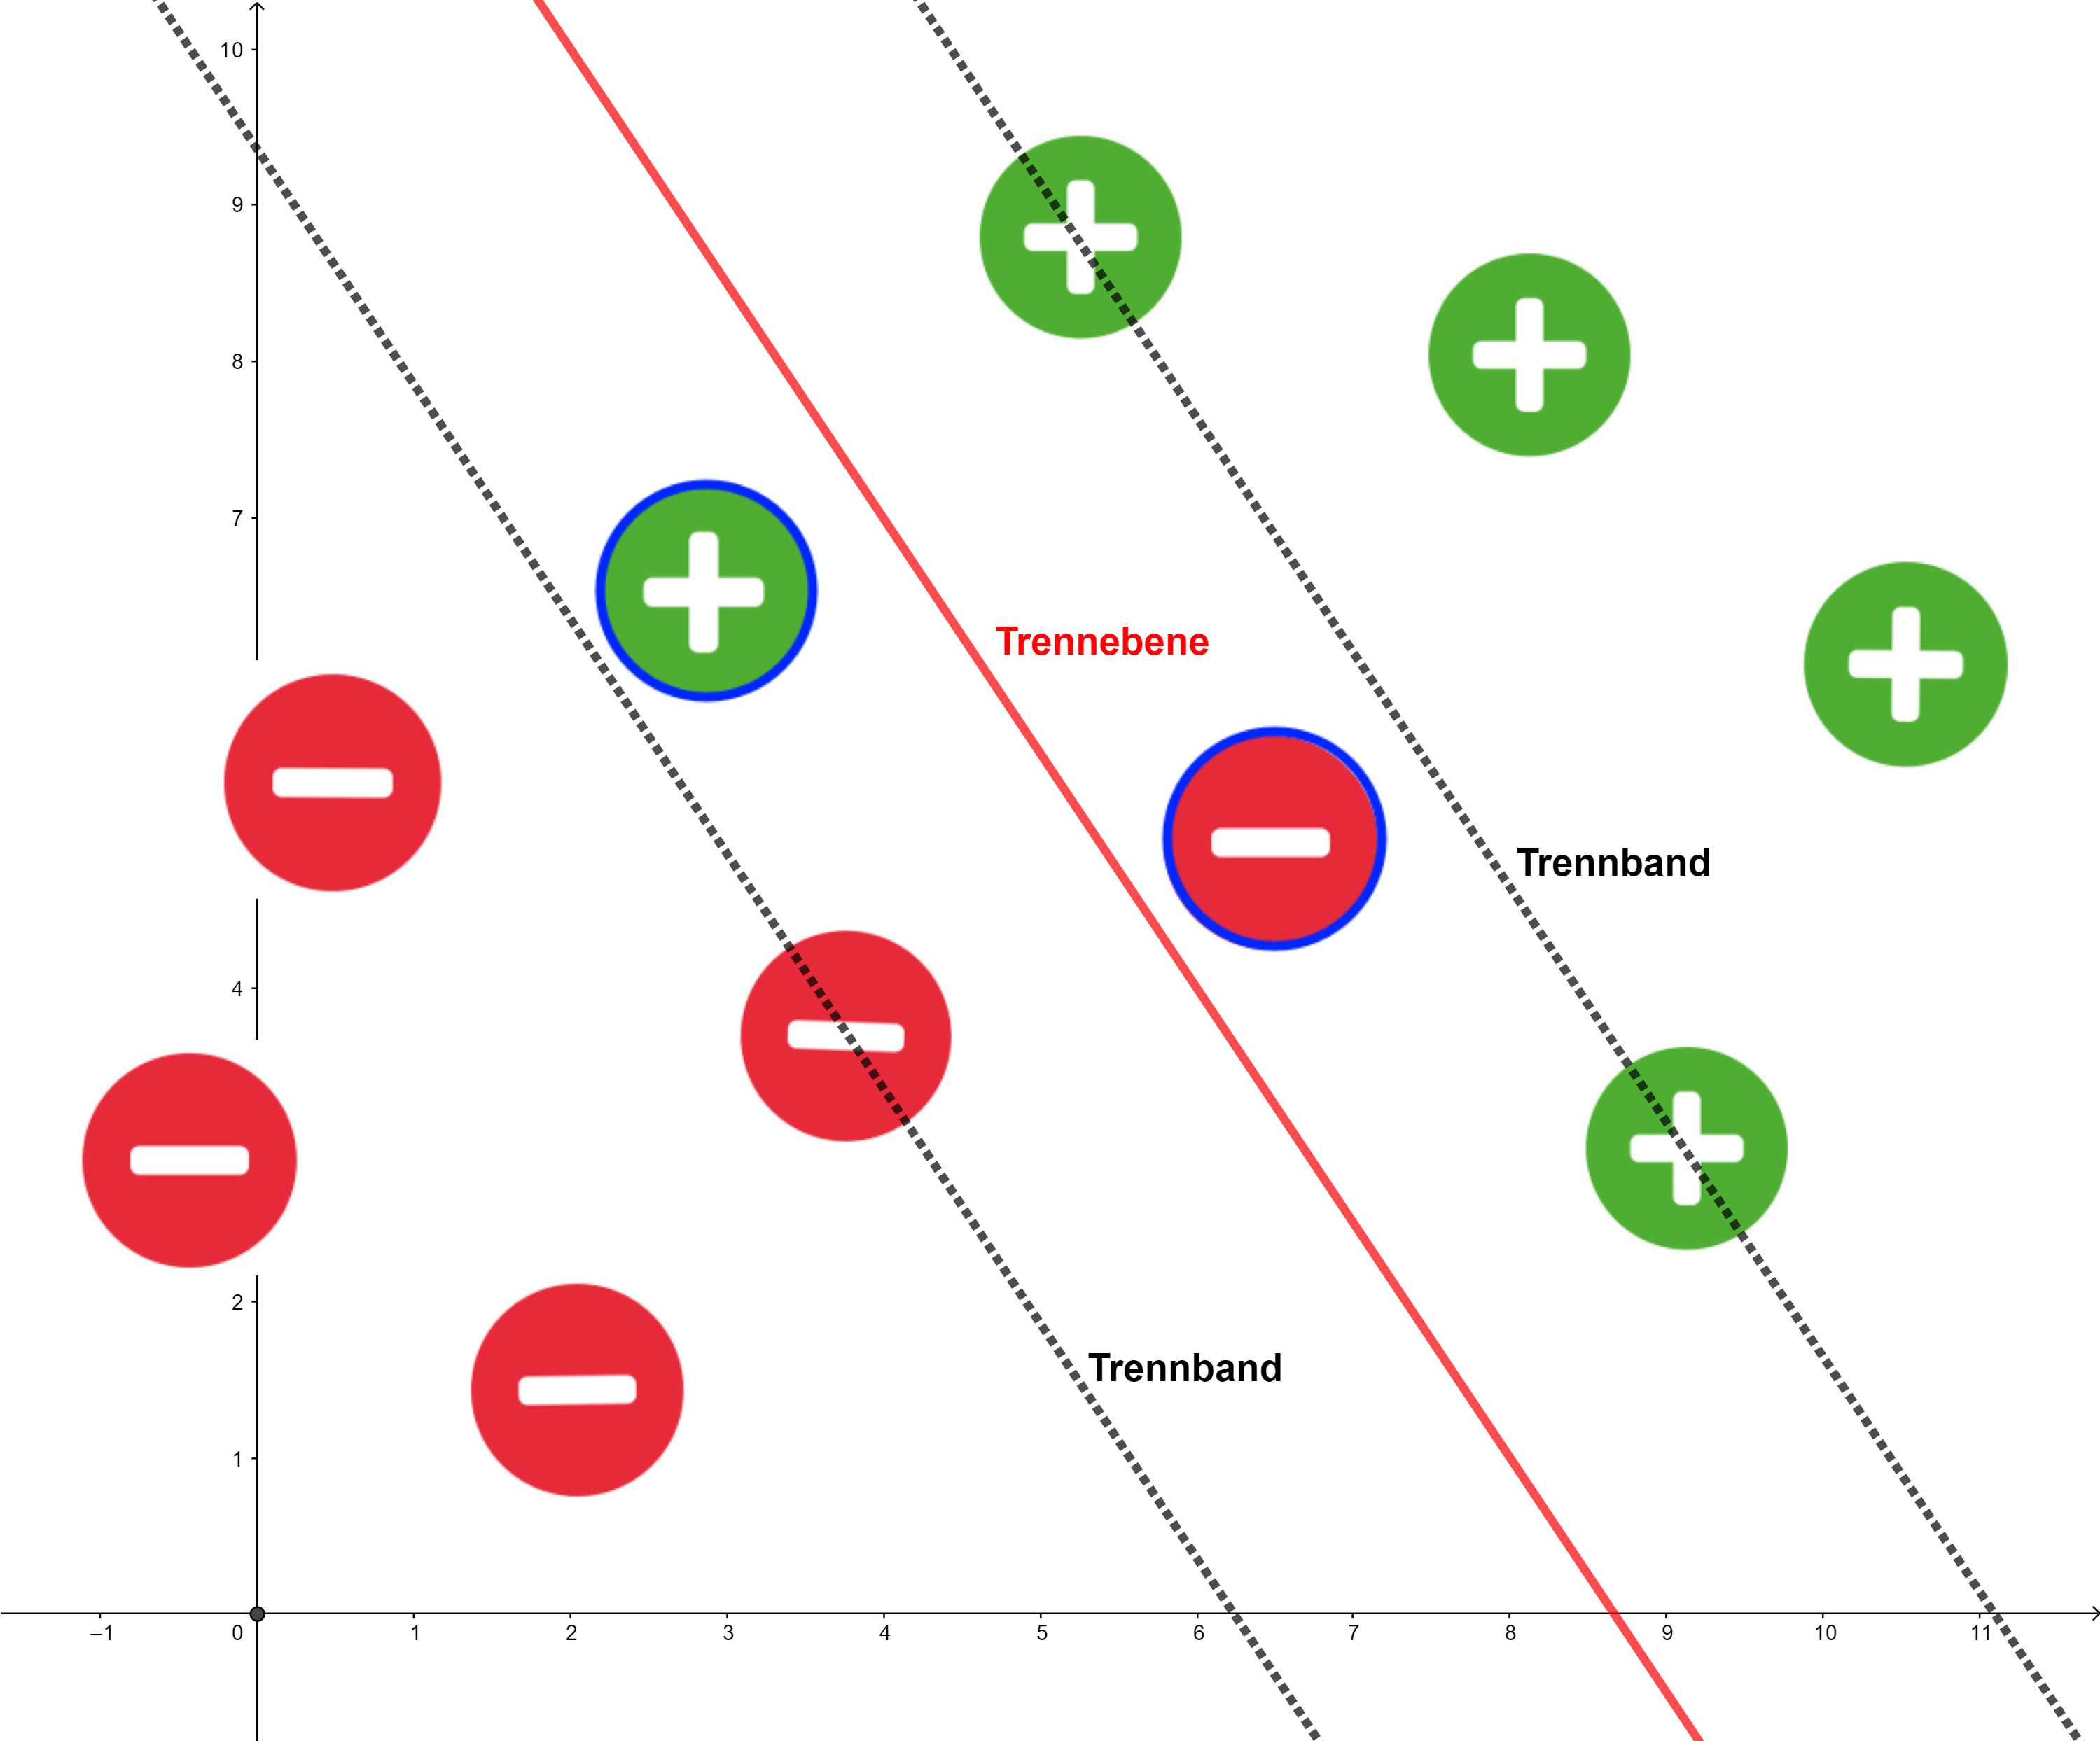
\includegraphics[width = 12cm]{assets/soft_margin_example.png}
	\caption{Die Eingabevektoren können nicht ohne einzelne Fehlklassifizierungen (blau markiert) linear getrennt werden.}
	\label{fig:soft_margin_example}
\end{figure}

In den Überlegungen in \autoref{sec:hard_margin} wurde angenommen, dass alle Eingabevektoren linear separierbar sind ohne dass Fehlklassifikationen aufreten. Dieses Problem kann durch eine Hard-Margin \ac{SVM}, wie in den Kapiteln zuvor gezeigt, gelöst werden. Trifft diese Annahme für eine Menge von Eingabevektoren nicht mehr zu, wie in \autoref{fig:soft_margin_example} dargestellt, kann der bisher beschriebene Algorithmus keine lineare Trennebene finden. Durch die Einführung von positiven Fehlervariablen $\xi_{n} \in \mathbb{R}^{K}, \xi_{n} \geq 0$ in \autoref{decision_rules} kann dieses Problem umgangen werden und trotzdem eine fehlerbehaftete, lineare Trennebene gefunden werden:

\begin{subequations} \label{decision_rules_softmargin}
	\begin{alignat}{2}
		w^{T} x_{n} + b \geq +1 - \xi_{n}& \qquad & \text{ für } y_{n} = +1\\
		w^{T} x_{n} + b \leq -1 + \xi_{n}& & \text{ für } y_{n} = -1
	\end{alignat}
\end{subequations}


Damit ein Eingabevektor $x_{n}$ nun, gemäß \autoref{decision_rules_softmargin}, falsch klassifiziert werden kann muss der zu dem Vektor gehörende Fehler $\xi_{n}$ über $1$ steigen. Eine obere Grenze für die Anzahl der aufgetretenen Fehler kann somit beschrieben werden durch $\sum_{n=1}^{N} \xi_{n}$. \\

Basierend auf dieser Grundlage kann eine Kostenfunktion $E$ basierend auf der Anzahl der Fehler formuliert werden:
\begin{equation} \label{soft_margin_error_cost_function}
	\begin{aligned}
		E = C(\sum_{n=1}^{N} \xi_{n})
	\end{aligned}
\end{equation}

Der Parameter $C \in \mathbb{R}, C \geq 0$ bestimmt die Höhe der Bestrafung von Fehlern und kann frei gewählt werden. \\


Erweitert man die zu minimierende Funktion $\frac{1}{2} w^{T} w $ aus \autoref{min_problem} um die Kostenfunktion $C(\sum_{n=1}^{N} \xi_{n})$ so erhält man ein neues Optimierungsproblem:

\begin{subequations} \label{soft_margin_problem}
	\begin{alignat}{2}
		&\!\min_{w}        &\qquad&  \frac{1}{2} w^{T} w + C(\sum_{n=1}^{N} \xi_{n}) \label{eq:optProbsoft}\\
		&\text{mit } &      & y_n (w^{T} x_{n} + b)-1 \geq 0 \text{ für } n=1..N \label{eq:constraintsoft}
	\end{alignat}
\end{subequations}

Wendet man die in \autoref{sec:lagrange} beschriebenen Schritte auf das in \autoref{soft_margin_problem} beschriebene Problem an erhält man folgendes Optimierungsproblem:

\begin{subequations} \label{final_lagrange_soft}
	\begin{alignat}{2}
		&\!\max_{\alpha}        &\qquad&  	\Lagr(\alpha) = \sum_{n=1}^{N} \alpha_{n} - \frac{1}{2} \sum_{n=1}^{N} \sum_{m=1}^{M} y_{n} y_{m} \alpha_{n} \alpha_{m} x_{n}^{T} x_{m} \label{eq:soft_margin_final}\\
		&\text{mit } &      & 0 \leq \alpha_{n} \leq C \text{ für } n=1..N \label{eq:constraint_soft}\\
		&       & & \sum_{n=1}^{N} \alpha_{n} y_{n} = 0\text{ für } n=1..N
	\end{alignat}
\end{subequations}

Sehr bemerkenswert hier ist, dass der einzige Unterschied zu \autoref{final_lagrange} die Beschränkung der Lagrange Multiplikatoren durch $C$ ist. Umgekehrt bedeutet dies, dass eine Hard-Margin SVM durch \autoref{final_lagrange_soft} beschrieben werden kann wenn der Parameter $C$ sehr groß gewählt wird.


\section{Nichtlineare Trennung}

TODO: text here

\subsection{Transformation der Problemstellung in eine höhere Dimension}
Idee: nichtlineare Transformation der Eingabevektoren in beliebig hohe, endliche Dimension \\

Transformation $\Phi(x): \mathbb{R}^{K} \rightarrow \mathbb{R}^{L}$ \\

Statt $x$ wird $\Phi(x)$ überall eingesetzt -> 

\begin{subequations} \label{eq:soft_margin_with_transform}
	\begin{alignat}{2}
		&\!\max_{\alpha}        &\qquad&  	\Lagr(\alpha) = \sum_{n=1}^{N} \alpha_{n} - \frac{1}{2} \sum_{n=1}^{N} \sum_{m=1}^{M} y_{n} y_{m} \alpha_{n} \alpha_{m} \Phi(x_{n})^{T} \Phi(x_{m})\\
		&\text{mit } &      & 0 \leq \alpha_{n} \leq C \text{ für } n=1..N\\
		&       & & \sum_{n=1}^{N} \alpha_{n} y_{n} = 0\text{ für } n=1..N
	\end{alignat}
\end{subequations}

Wie in \autoref{eq:soft_margin_with_transform} ersichtlich: Einzige Zusatzkosten sind höherdimensionale Skalarprodukte in Optimierung. Anzahl Alphas und Dimension der Q-Matrix aus \autoref{qp1} bleibt gleich weil diese nur abhängig von Anzahl Testdaten sind und nicht von der Dimension.\\

Generalisierungsverhalten beurteilen: Anzahl SV dividiert durch Anzahl Testdaten -> möglichst kleine Zahl \\

Vorschau: Bei Kernel-Trick: sogar Kosten für Skalarprodukt erspart

\subsection{Kernel Methode}



% THIS COMMAND ADDS ALL ENTRIES (EVEN UNREFERENCED) TO BIBLIOGRAPHY
\nocite{*}

% Literaturverzeichnis:
\clearpage
\phantomsection
\addcontentsline{toc}{chapter}{Bibliography}
\printbibliography

\end{document}
